% !Mode:: "TeX:UTF-8"
% !TEX program  = xelatex

\documentclass[dvipsnames,withoutpreface,bwprint]{cumcmthesis}
\usepackage[framemethod=TikZ]{mdframed}
\usepackage{url}   % 网页链接
\usepackage{subcaption} % 子标题
\usepackage{float}%把figure环境变为不浮动状态
\usepackage{placeins}
\usepackage{enumitem}
\usepackage{calc}
\usepackage{pifont}%带圈数字的宏包
\usepackage{multirow,makecell}%划分表格使用的宏包
\usepackage{xcolor}%颜色盒子所用的宏包
\usepackage{cite}
\usepackage{ctex}
\title{基于模糊数学的中小微企业信贷决策模型}
\tihao{C}
\baominghao{}
\schoolname{}
\membera{}
\memberb{}
\memberc{}
\supervisor{}
\yearinput{2020}
\monthinput{5}
\dayinput{5}
\renewcommand{\refname}{}
\renewcommand{\upcite}[1]{\textsuperscript{\textsuperscript{\cite{#1}}}} %参考文献右上角小标
\begin{document}
\maketitle
\begin{abstract}
自2014年9月夏季达沃斯论坛上李克强总理提出,要在960万平方公里土地上掀起“大众创业”、“草根创业”的新浪潮以来,越来越多的中小微企业挺地而起。而中小微企业的创业途中,银行的贷款往往是其现金流中不可或缺的一部分。因此,在中小微企业泛滥的大环境下,银行制定合理的中小微企业信贷决策模型对于保证银行的利益变得尤为重要。\\
\indent\textbf{针对问题一:}研究银行的信贷策略,主要考虑信贷额度和信贷利率的制定。信贷额度的计算主要是通过建立六个指标,并对此六个指标进行\textbf{无量纲化},建立\textbf{最优化模型},使得银行的利润最大化,通过python对附件1中所给的进行一系列数据进行\textbf{线性拟合},计算出其六项指标的无量纲值,之后使用\textbf{层次分析法}对所有指标进行处理,即可得出银行的放贷金额。而信贷利率的计算主要利用附件1中所提供的不同信誉等级的企业的流失率随着贷款年利率的升高而降低,因此便考虑使用\textbf{迭代求解}方法,来求解不同信誉等级的企业所对应的贷款年利率。\\
\indent\textbf{针对问题二:}由于302家企业的信誉等级是未知的,因此我们通过附件1的123家企业的发票信息以及其对应的信誉等级建立\textbf{置信区间},用其来预测302家企业的信誉等级,之后便使用问题一中建立的模型进行求解即可。\\
\indent\textbf{针对问题三:}本题在问题二的基础上多考虑了突发因素对生产经营和经济效应的影响,因此银行在给企业放贷前应该将企业的负载能力作为一个比较重要的指标,而负载能力与企业的能承受的最大欠款以及扭亏为盈所花费的时间是息息相关的,所以本题需要在问题一的基础上,将企业负载能力所占的权重提高即可。\\
\
\indent\textbf{关键词:}\quad 无量纲化\quad 线性拟合\quad 层次分析法\quad 迭代法\quad 置信区间
\end{abstract}
\section{问题背景与重述}
\subsection{问题背景}
\par 随着我国经济市场化程度的加深,银行和企业的理性程度、信贷利率市场化程序也在不断地提高,但小企业贷款难的状况依然存在。通过解决银行和企业等理性主体之间的信贷博弈和信贷市场存在的矛盾,结合相关因素的定性与定量分析,在拥有充分的资料和可靠的信息下,
把银行贷款的风险降到最大,把企业贷款的金额最大化,提出相应的信贷决策。在这样的模型下为银行信贷风险管理提供科学的决策理论和方法,无疑是至关重要的。
\subsection{问题重述}
\par 在实际中,由于中小微企业规模相对较小,也缺少抵押资产,因此银行通常是依据信贷政策、企业的交易票据信息和上下游企业的影响力,向实力强、供求关系稳定的企业提供贷款,并可以对信誉高、信贷风险小的企业给予利率优惠。
银行首先根据中小微企业的实力、信誉对其信贷风险做出评估,然后依据信贷风险等因素来确定是否放贷及贷款额度、利率和期限等信贷策略。
\par 某银行对确定要放贷企业的贷款额度为10 \textasciitilde 100万元;年利率为4\% \textasciitilde 15\%;贷款期限为1年。
附件1 \textasciitilde 3分别给出了123家有信贷记录企业的相关数据、302家无信贷记录企业的相关数据和贷款利率与客户流失率关系的2019年统计数据。该银行请你们团队根据实际和附件中的数据信息,通过建立数学模型研究对中小微企业的信贷策略,主要解决下列问题:
\begin{enumerate}[fullwidth,itemindent=2em,label=(\arabic*)]
    \item 对附件1中123家企业的信贷风险进行量化分析,给出该银行在年度信贷总额固定时对这些企业的信贷策略。
    \item 在问题1的基础上,对附件2中302家企业的信贷风险进行量化分析,并给出该银行在年度信贷总额为1亿元时对这些企业的信贷策略。
    \item 企业的生产经营和经济效益可能会受到一些突发因素影响,而且突发因素往往对不同行业、不同类别的企业会有不同的影响。综合考虑附件2中各企业的信贷风险和可能的突发因素(例如:新冠病毒疫情)对各企业的影响,给出该银行在年度信贷总额为1亿元时的信贷调整策略。
\end{enumerate}
\section{问题分析}
\subsection{问题一的分析}
对于问题一,我们需要通过附件1给出的123家企业的信贷记录对其信贷风险进行量化分析,而不同企业的信贷风险不同也决定了银行愿意给出企业的贷款额度。由于各项财务指标并不容易确定,也难以通过某一标准来进行企业风险的量度,对此我们采用如下三个指标来给银行制定贷款策略。
\par 指标一是判断是否给该企业放贷,我们直接给出贷款门槛,即有过违约的记录一律不放贷,可筛选出部分企业;指标二是对于守约的企业银行给出的贷款额度,其受信用评级和盈利能力、负载能力影响,
盈利能力是指企业开具的销项发票中获得的利益,负载能力是指企业在交易过程中能承受的最大额度,由最大盈利减去最大亏损得到;指标三是指银行给企业的贷款利率,取决于不同信用评级下对应的利率和客户流失率最大化,
在利率增加的情况下客户的流失率必然增加,找到一个合适的比例得出贷款利率使得银行企业双方实现共赢。
\subsection{问题二的分析}
在问题二中,由于并没有此302家企业的信用评级和守约记录图,因此我们采用统计学上的置信区间来划分D等级的企业,可直接排除D级企业的信贷策略,另有企业的进项和销项发票,对此我们可以在问题一的基础上重新建模,考虑从企业的盈利能力入手,盈利能力在问题一的基础上我们增加了其盈利曲线的斜率和方差关系,斜率的变化代表着企业盈利的速率快慢,
有可能该企业的资产并不大,但是具有巨大的盈利潜力,银行也可考虑放贷。方差反映了数据和平均值的偏离程度,即反映了企业盈利的稳定程度,若企业长时间盈利后又亏损反反复复不稳定,银行也得酌情考虑放贷额度。
\subsection{问题三的分析}
在问题三中,考虑到企业的生产经营和经济效益可能会受到一些突发因素影响,企业很有可能无法收回本金,造成银行的损失。因此银行在对企业的信贷风险进行量化分析时,应该把企业的负载能力的优先级提升到一个比较高的位置,保证企业的负载能力能够换的上银行所放出的贷款,保证银行的基本利益。
\section{模型假设}
\begin{enumerate}
    \item 假设银行给企业的信用评级在我们的研究时间段不会发生转变。
    \item 假设进项发票中的税额并不由该企业给出。
    \item 假设题目所给的数据真实可靠。
\end{enumerate}
\section{符号说明}
\begin{table}[H]
    \renewcommand\tabcolsep{2cm} % 调整表格列间的宽度
    \begin{tabular}{@{\quad} ccc @{\qquad}@{\quad}}
        \toprule[1.5pt]
        符号 & 说明 & 单位\\
        \midrule[1.5pt]
        $x_i$ & 第i家企业的平均每月盈利情况 & 元\\
        $a_i$ & 第i家企业的收入情况 & 元\\
        $b_i$ & 第i家企业的支出情况 & 元\\
        $s_{ij}$ & 第i家企业在j时刻的盈利情况 & 元\\
        $T_i$ & 第i家企业有发票记录的月份总数 &个\\
        $t_i$ & 第i家企业的盈利月份 &{}\\
        $f_i$ & 第i家企业的最大负载能力 &元\\
        $r_i$ & 银行给第i家企业的放款额度 &元\\
        $R_i$ &第i家企业扭亏为盈的最长时间 &月\\
        $m_i$ &第i家企业的收入稳定度 &{}\\
        $n_i$ &第i家企业的支出稳定度 &{}\\
        $\gamma$ & 风险指标 &{}\\
        $\delta$ & n等级下的理论收益指数 &{}\\
        $\alpha_n$ & n等级下的贷款利率 &{}\\
        $\beta_n$ & n等级下的客户流失率 &{}\\
        \bottomrule[1.5pt]
    \end{tabular}
\end{table}
\section{模型的建立与求解}
\subsection{研究意义}
自2014年9月夏季达沃斯论坛上李克强总理提出,要在960万平方公里土地上掀起“大众创业”、“草根创业”的新浪潮以来,越来越多的中小微企业挺地而起。而中小微企业的创业途中,银行的贷款往往是其中不可或缺的一部分。因此,在中小微企业泛滥的大环境下,银行建立对企业的放贷策略模型迫在眉睫。
\subsection{建模方法介绍}
\subsubsection{层次分析法}
\par 层次分析法(简称AHP)是美国运筹学家Saaty教授于20世纪70年代初提出的,其特点是把复杂问题中的各种因素通过划分为相互联系的有序层次,使之条理化。作为规划、决策和评价的工具,AHP自问世以来,已在各个领域得到迅速普及和推广,取得了大量的研究成果。
层次分析法主要用于确定综合评价的权重系数,所用数学工具主要是矩阵的运算。信用风险的测算是一个复杂的、多层次的评价过程,每个指标要素之间的关系是相互依存、相互作用的,它们是一个整体。
\subsubsection{置信区间}
\par 置信区间是指由样本统计量所构造的总体参数的估计区间。在统计学中,一个概率样本的置信区间(Confidence interval)是对这个样本的某个总体参数的区间估计。置信区间展现的是这个参数的真实值有一定概率落在测量结果的周围的程度,其给出的是被测量参数的测量值的可信程度,即前面所要求的“一个概率”。
\subsubsection{迭代法}
\par 迭代法也称辗转法,是一种不断用变量的旧值递推新值的过程,跟迭代法相对应的是直接法(或者称为一次解法),即一次性解决问题。迭代算法是用计算机解决问题的一种基本方法,它利用计算机运算速度快、适合做重复性操作的特点,让计算机对一组指令(或一定步骤)进行重复执行,
在每次执行这组指令(或这些步骤)时,都从变量的原值推出它的一个新值,迭代法又分为精确迭代和近似迭代。比较典型的迭代法如“二分法”和"牛顿迭代法”属于近似迭代法。
\subsection{问题一模型的建立}
对于银行来说,对中小微企业的放贷额度由平均每月盈利、收入稳定性、支出稳定性、最大负载能力、最长扭亏转盈时间、信用评级所决定。对于有信贷记录的123家企业而言,银行原则上不会给D级以及B、C中违约的企业发放贷款,仅对未产生违约行为的企业发放贷款,对表格中的违约企业进行筛选,得知A级信用评级的企业没有违约的,B级中有一个,C级有2个,D级是全部违约了的。
\par 由于问题一一共有123家企业,将银行对于每一家企业的贷款策略都是不同的,因此本文只选取了企业E6作为我们的目标对象,至于123家企业的详细贷款额度和贷款利率,请查阅支撑材料中的《1题信贷额度.xls》。对于以下的讨论,我们以$E_6$企业为参考,可以绘制出我们的思路流程如下图所示:
\begin{figure}[H]
    \centering
    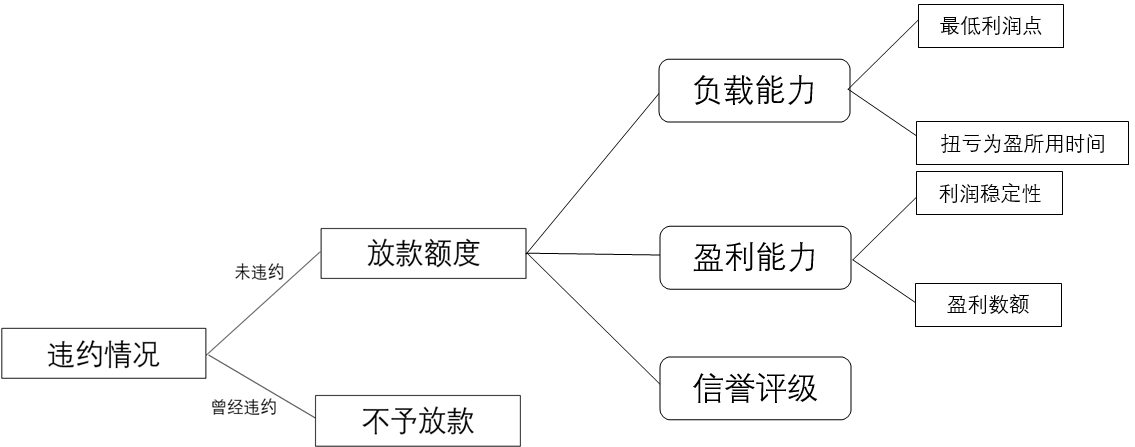
\includegraphics[width=.9\textwidth]{figure-3.png}
    \caption{模型思路流程图}
    \label{fig:1}%交叉引用标签
\end{figure}
\subsubsection{企业平均盈利情况的确定}
通过python编程引入守约企业所给的进项和销项发票数据,得到企业收入和支出的情况,由此得出企业的盈利情况,即:
\begin{equation}
    s_i=a_i-b_i \quad i=1,2\dots123
\end{equation}
\par 通过上述函数编程代入数据得到企业的盈利情况,由此得出平均每月盈利如下:
\begin{equation}
     x_i=\frac{s_i}{T_i} \quad i=1,2\dots123
\end{equation}
\par 具体每个企业的每月盈利情况请查看支撑材料《1题企业月净利润.xls》。
\subsubsection{收入稳定性和支出稳定性的确定}
稳定性由方差反映出来,具体的收入方差请查看支撑材料《1题企业月进项方差.xls》。对于盈利的企业来说,收入的稳定性越低越好,对于亏损的企业来说,支出的稳定性越大越好,因为对于亏损的企业来说,他的目的只想盈利,若企业越不稳定则越有可能获利,建立以下数学模型:
\begin{gather}
    m_i=\frac{1}{n} \cdot \sum\limits _{i=1}^n (a_i-\overline{a_i})^2\\
    n_i=\frac{1}{n} \cdot \sum\limits _{i=1}^n (b_i-\overline{b_i})^2\\
    i=1,2\dots123 \notag
\end{gather}
\subsubsection{最大负载能力的确定}
企业在经营的过程中必定会出现盈利情况的上下起伏,而企业能够承受的最大负载能力即有交易记录最近月份的资产与历史最低资产的差值成为评判该企业能力的一项指标,若企业的负载能力较大,则说明该企业在遇到突发情况下的抗风险能力较强。建立出以下数学模型:
\begin{equation}
    f_i=s_{i(new)}-s_{i(low)}\quad i=1,2\dots123
\end{equation}
\par 其中$s_{i(new)}$表示有交易记录最近月份第i家企业的盈利情况,$s_{i(low)}$表示第i家企业历史盈利情况最低的时候,$f_i$即表示第i家企业的最大负载能力。如下图为$E_6$企业的最大负载能力图。
\begin{figure}[H]
    \centering
    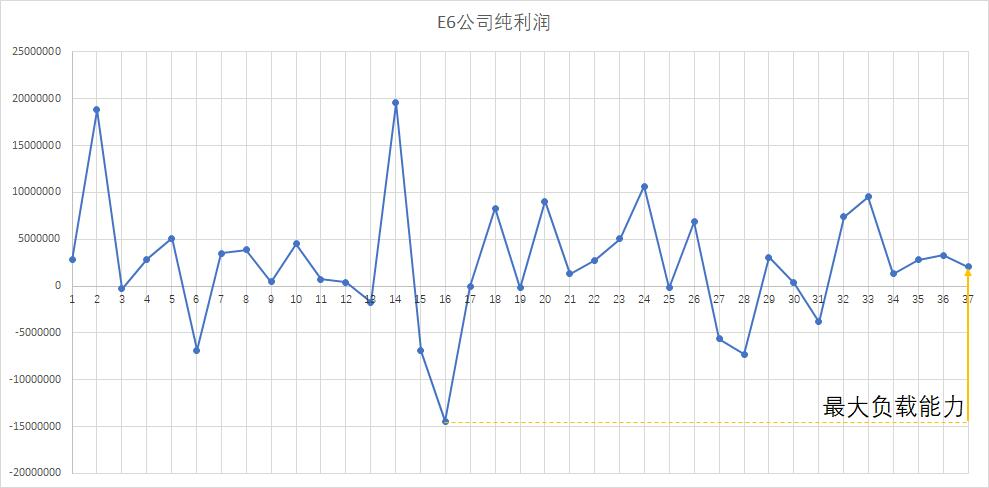
\includegraphics[width=.9\textwidth]{figure-4.jpg}
    \caption{$E_6$企业的最大负载能力}
    \label{fig:2}%交叉引用标签
\end{figure}
\par 由此我们可以直观的得出该企业的最大负载能力为:3998279.4。至于123家企业的具体最大负载能力,请查看支撑材料《1题企业最大负载能力.xls》。
\subsubsection{最长扭亏转盈时间的确定}
在企业经营的过程中,有的企业可能会一直亏损无法盈利而最终导致破产,而企业如何在更快的时间里从亏损的情况下回到盈利,成为评判该企业能力的一项指标,我们称此时间为最长扭亏转盈时间,该时间由盈利曲线的两驻点位置所确定,所以我们应建立盈利曲线的导数方程:
\begin{equation}
    R_i=\frac{\mathrm{d}si}{\mathrm{d}ti}=0\quad i=1,2\dots123
\end{equation}
\par 其中$s_i$表示第i家企业的盈利曲线,$t_i$表示第i家企业的盈利月份时间,对该曲线进行求导等于0的时刻即为该曲线的驻点,而两驻点之间间隔的时间即是我们所求的扭亏转盈的时间,再通过python编程算出两两驻点之间的间隔时间,求出最大值,重复123次,便可得到123家企业的最长扭亏转盈时间。如下图为$E_6$企业的最长扭亏转盈时间图。
\begin{figure}[H]
    \centering
    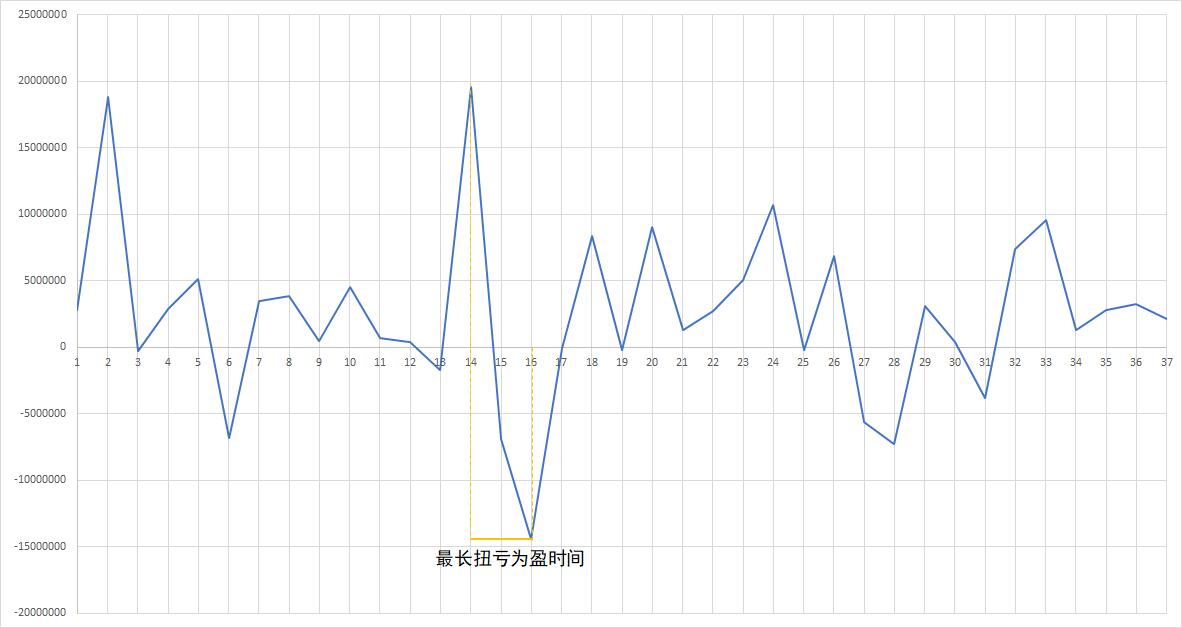
\includegraphics[width=.9\textwidth]{figure-5.jpg}
    \caption{$E_6$企业的最长扭亏转盈时间}
    \label{fig:3}%交叉引用标签
\end{figure}
\par 由此我们可以直观的得出该企业的最长扭亏转盈时间为:两个月。至于123家企业的具体最长扭亏转盈时间,请查看支撑材料《1题企业最长扭亏转盈时间.xls》。
\subsubsection{信用评级带来的风险指标确定}
银行对于不同企业给出的信用评级,会影响其放款额度的指标,我们把这项指标称为风险指标。对于A,B,C三个等级,银行放款的时候,会给予不同的权重,此权重不容易被量化,因此我们采用层次分析法来分配其权重。
\par 假设函数$f(x,y)$,表示评价指标x对于评价指标y的重要程度,约定$f(x,y)=1/f(y,x)$,即可求得下表: 
\begin{table}[H]   
    \caption{层次分析法的重要程度指标}
    \resizebox{\textwidth}{!}{
    \begin{tabular}{|c|c|c|}
        \hline
        重要程度 &说明 &f(x,y) \\\hline
        x与y同等重要 &x,y对总指标有相同的重要程度 &1 \\\hline
        x比y稍微重要 &x的重要程度大于y,但是不明显 &3 \\\hline
        x比y明显重要 &x的重要程度明显大于y,但不十分明显 &5 \\\hline
        x比y非常重要 &x的重要程度十分大于y,但不特别突出 &7 \\\hline
        x比y绝对重要 &x的重要程度以压倒优势大于y &9 \\\hline
        x与y介于各等级之间 &相邻两判断的折中 &2,4,6,8 \\\hline
    \end{tabular}}
\end{table}
目标层为风险指标,准则层为违约率,负载能力,信用评级,方案层为A,B,C。
如下图所示:
\begin{figure}[H]
    \centering
    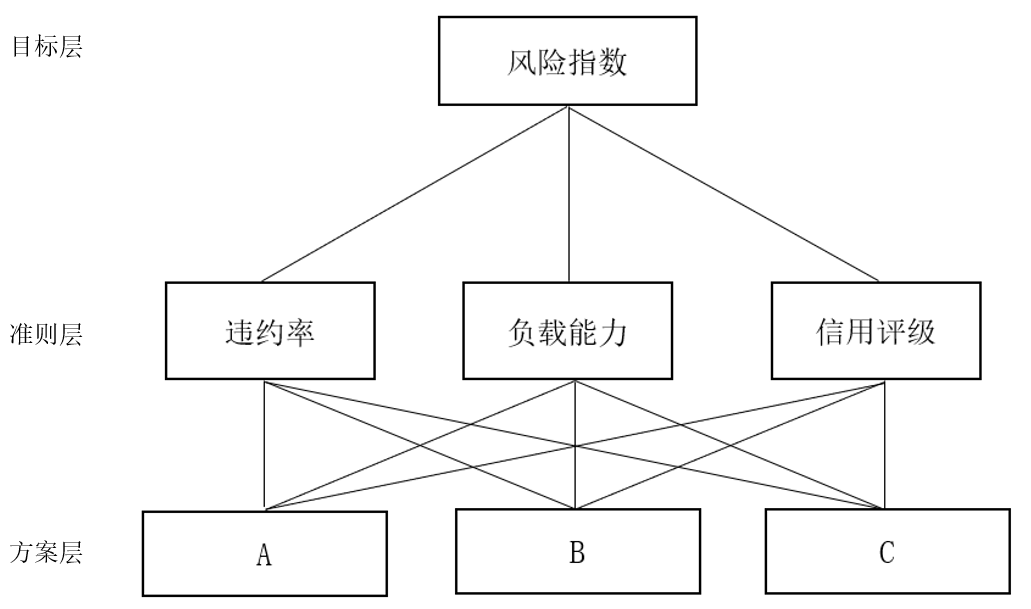
\includegraphics[width=.8\textwidth]{figure-1.png}
    \caption{风险指标的层次结构模型}
    \label{fig:2}%交叉引用标签
\end{figure}
\begin{enumerate}[label=(\arabic*)]
    \item 构造判断矩阵
    \par \qquad 因为判别元素的值反映了综合评价指数对各因素相对重要程度的认识,根据上述表格来建立因子之间的重要程度,得出构造矩阵$C=(c_{ij})_{n \times n}$,其中$c_{ij}=f(x_i,x_j)$。
    \[C=\begin{bmatrix}
        c_{11} &\dots &c_{15} \\
        & \ddots & \vdots \\
        c_{51} & &c_{55} \\
    \end{bmatrix}\]
    对准则层三个指标进行重要程度控制,得到以下矩阵:
    \[C=\begin{bmatrix}
        1 &1/5 &3 \\
        5 &1 &5 \\
        1/3 &1/5 &1 \\
    \end{bmatrix}\]
    \item 层次单排序及其一致性检验
    \par \qquad 通过判别矩阵C的特征根求解$(CW=\lambda W)$得到特征向量W ,经过归一化后即得同一层次响应因素对于上一层次因素相对重要性的排序权值,即进行层次单排序。
    \par 根据一致性检验指数$CI=\lambda-n/n-1$,若通过一致性检验则合理。采用matlab编程,具体代码见附录A,得到归一化后的特征向量$\gamma_1$为
    \[\begin{bmatrix}
            0.0972,0.2021,0.7007
    \end{bmatrix}\]
    即为A,B,C三种等级的企业的风险指标,由此可见给评级为A的企业贷款的风险最低,故A等级在借贷的时候放款金额具有一定的优势。
\end{enumerate}
\subsection{问题一模型的求解}
\subsubsection{信贷额度的分配}
通过以上分析我们确定了六个指标:平均每月盈利、收入稳定性、支出稳定性、最大负载能力、最长扭亏转盈时间、信用评级,通过这六个指标得到银行给予的信贷额度,而如何权衡这六个指标的重要程度,到底孰轻孰重,成为得出最终方案的关键,我们再次采用层次分析法进行求解。
\par 目标层为信贷额度,准则层为平均每月盈利,收入稳定值,支出稳定性,最大负载能力,最长扭亏为盈时间,信用评级,方案层为A,B,C,我们建立的重要程度为平均每月盈利>最大负载能力>最长扭亏转盈时间>稳定性>信用评级,如下图所示:
\begin{figure}[H]
    \centering
    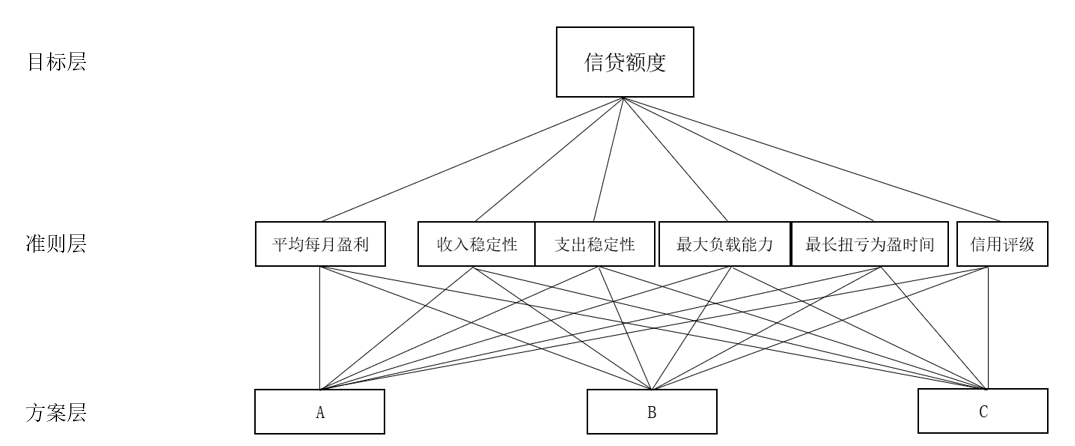
\includegraphics[width=.9\textwidth]{figure-2.png}
    \caption{信贷额度的层次结构模型}
    \label{fig:3}%交叉引用标签
\end{figure}
判断矩阵如下:
\[C=\begin{bmatrix}
    1 &7 &7 &2 &5 &9 \\
    1/7 &1 &1 &1/4 &1/3 &3 \\
    1/7 &1 &1 &1/4 &1/3 &3 \\
    1/2 &4 &4 &1 &3 &7 \\
    1/5 &3 &3 &1/3 &1 &6 \\
    1/9 &1/3 &1/3 &1/7 &1/6 &1
\end{bmatrix}\]
\par 采用matlab编程,得到特征向量$\gamma_2$为:
\[\begin{bmatrix}
    0.3966    ,0.0900   ,0.0900   ,0.2486   ,0.1336   ,0.0411
\end{bmatrix}\]
\par 由此我们得到了此六项指标所占的权重。
\subsubsection{信贷利率的分配}
由于贷款利率和客户流失率在附件3:银行贷款年利率与客户流失率关系的统计数据.xlsx中已经给出,可以很明显的观察到两者是一一对应的关系,并且随着贷款年利率的上升,客户流失率也在上升,如何平衡这二者的关系使得信贷利率与客户流失率的比值最大化,是确定其指数的关键。
\begin{equation}
    \delta =\alpha_n \cdot(1-\beta_n) \quad n=A,B,C
\end{equation}
\par 其中$\delta$我们称其为银行理论收益指数,$\alpha_n$为信贷利率,$\beta_n$为流失率。
\subsubsection{目标函数及约束条件}
我们确定了六个指标,并划分了每一个指标的权重,但是这六个指标的量纲并不相同,使得两两之间不具有可比较性,因此我们对数据进行无量纲化处理,消除量纲后建立出目标函数和约束条件。
\[\text{目标函数:}maxZ=\delta\cdot \begin{bmatrix}\gamma_2\end{bmatrix}\begin{bmatrix}x_i&m_i&n_i&f_i&R_i&\gamma_1 \end{bmatrix}^ \mathrm{ T }\]
\begin{equation}
    s.t \left\{
    \begin{aligned}
        &x_i=\frac{s_i}{T_i}\\
        &m_i=\frac{1}{n} \cdot \sum\limits _{i=1}^n (a_i-\overline{a_i})^2\\
        &n_i=\frac{1}{n} \cdot \sum\limits _{i=1}^n (b_i-\overline{b_i})^2\\
        &f_i=s_{i(new)}-s_{i(low)}\\
        &R_i=\frac{\mathrm{d}si}{\mathrm{d}ti}=0\\
        &\delta =\alpha_n \cdot(1-\beta_n)-d_n
    \end{aligned}
    \right.
    \label{equation:1}
\end{equation}
\par 目标函数的意思是六个指标乘以相应的权重然后相加即是信贷额度,再乘以不同等级对应的信贷利率,最后的数据就是我们划分信贷策略的依据。
\par 因为数据量过于庞大,所以我们采用python进行编程求解,代入附件1所给的进项和销项数据先算出每个企业的收入和支出得到$x_i$,由上文的层次分析法得到$\gamma$,最后得到目标函数的数值情况,即可求解出对于每一家企业的信贷策略,根据前文可以求解出的银行对企业E6的贷款额度为13.5878551095389万元,由于企业E6是A级信誉评级,因此其对应的贷款年利率为0.0465。
\subsection{问题二模型的建立}
\subsubsection{问题二具体思路}
由于问题二中的302家企业并没有信誉评级和违约记录,所以评定这302家企业的信誉等级成为了解题的关键。首先我们通过附件1所给出的123家企业信誉评级、有效发票和作废发票为基本数据,并排除交易记录样本较少的45家企业,
采用数理分析中置信区间,得出其置信区间的比例,为银行对企业的可信度,即可划分出302家企业的信用等级。考虑到现实情况,在此我们并不会将企业的信誉等级设定为A等级,银行对于放出的贷款首先是收回贷出的本金,其次才是收回相应的利息,而这些企业并没有信贷记录,
因此贸然将企业视为信誉等级A的企业可能会导致银行本金大量流失,这无疑会对银行造成巨大的损失,所以对A等级的划分应该建立在有多次借贷记录的基础上,在本问题中不做讨论。
\par 通过以上分析划分出302家企业的信用等级,就可在问题一模型的基础上进行建模,编程代入附件2所给出的进项和销项发票数据,得到302家企业的经营情况、离散程度、盈利能力,对此做出相应的信贷策略。
\subsubsection{问题二模型数据处理}
因为在求置信区间时,运用附件1的数据时,我们将样本过少的数据排除掉,因此在带入附件二的数据放入置信区间判定时,我们同样也将样本较少的公司单独分析得到其信用评级。
对于销项发票与进项发票数量少于3位数的,先单独拿出来,然后因为银行方发放贷款,除了考虑如何利益最大化以外,还要保证能收回贷款的本金及利息,因此我们优先考虑其销项发票上的金额,其次考虑进项发票上的金额,销项发票金额反映公司盈利能力,进项发票上的金额可以反映该公司的资金储备,因此,我们将样本较少的公司以销项发票、进项发票的金额与其最大负载能力进行对比,得到如下关系:\\
\indent A——进项金额大,销项金额大。\\
\indent B——进项金额小,销项金额大。\\
\indent C——进项金额大,销项金额小。\\
\indent D——进项金额小,销项金额小。
\subsection{问题二模型的求解}
我们将问题二的模型数据求解出后,直接代入问题一所求解出的模型即可得出结果,我们在此以企业E125为例,将其有效交易与无效交易的比率代入置信区间中,可以得出企业E125的信誉评级为C,接下来我们便可按照解决问题一的方式来求解此问题。
\subsubsection{$E_{125}$企业金额}
根据问题一建立的模型,通过置信区间划分等级后,我们选择$E_{125}$企业为研究对象,代入问题一模型中,编程实现得到该企业的进项金额和销项金额如下图所示:
\begin{figure}[H]
    \centering
    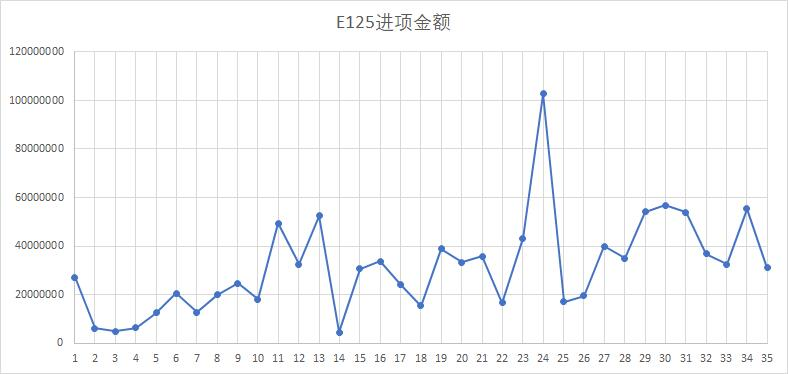
\includegraphics[width=.9\textwidth]{figure-6.jpg}
    \caption{$E_{125}$企业的进项金额}
    \label{fig:4}%交叉引用标签
\end{figure}
\begin{figure}[H]
    \centering
    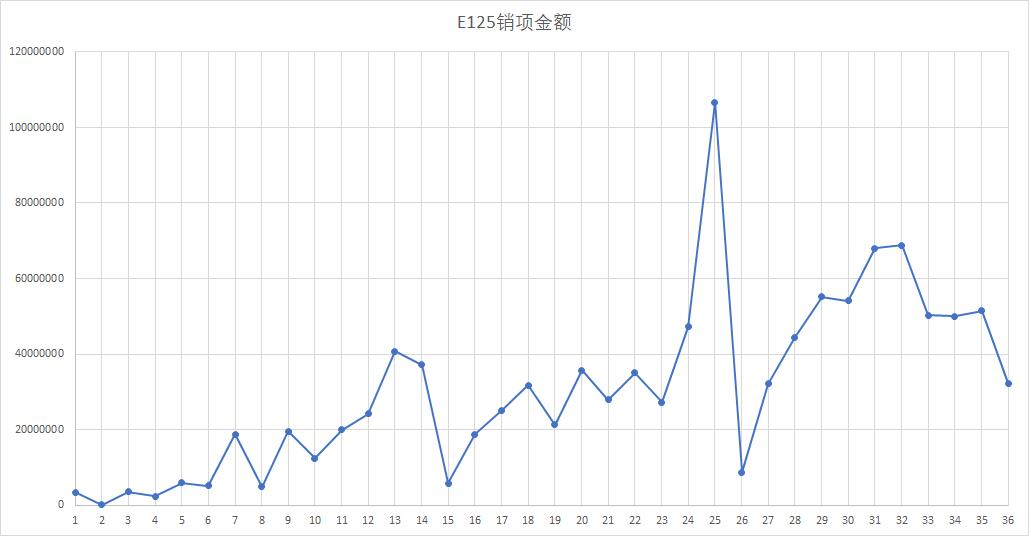
\includegraphics[width=.9\textwidth]{figure-7.jpg}
    \caption{$E_{125}$企业的销项金额}
    \label{fig:5}%交叉引用标签
\end{figure}
由以上图即可得到该企业的利润金额。
\begin{figure}[H]
    \centering
    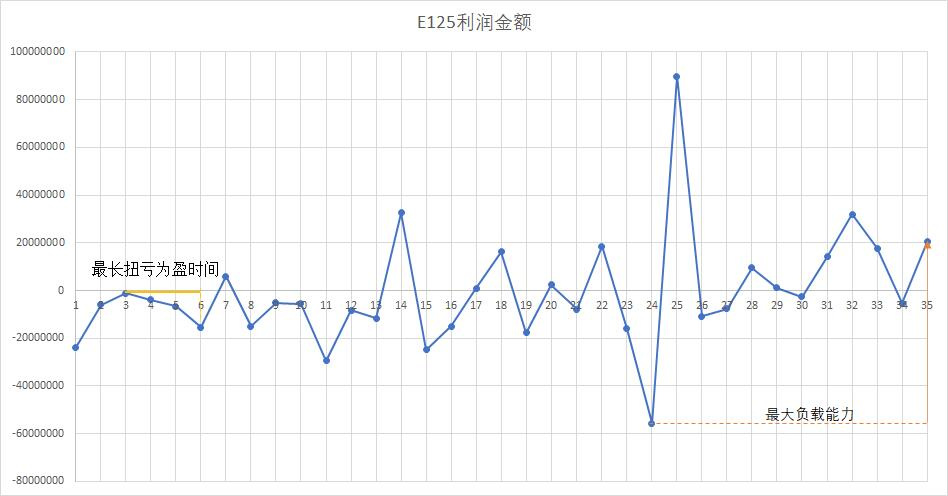
\includegraphics[width=.9\textwidth]{figure-8.jpg}
    \caption{$E_{125}$企业的利润金额}
    \label{fig:6}%交叉引用标签
\end{figure}
同股票该利润金额曲线可以直观的得到该企业的最长扭亏为盈的时间和最大的负载能力,因此就直接解决了问题一所提出的两项指标,同样的代入编程中即可得到企业E125的贷款额度为21.3352273877486元,贷款年利率为0.0585。至于其他的301家企业,请查阅支撑材料《2题企业信贷额度.xls》。
\subsection{问题三模型的建立与求解}
问题三讨论的是突发因素对企业的影响,显然突发因素的发生会对不同企业的盈利情况产生不同的作用,如发生新冠病毒疫情会造成线下的企业无法复工复产,使得工厂无法运作,而对于互联网企业来说,此时进行大数据分析以及相应的预测评判正是其工作的方向。
但是突发情况对不同企业造成的影响并不是我们可以研究的,这需要大量的市场调研以及参数指标来确定,而我们没有相应的资料,因此此影响因子不在我们考虑的范围之内。
\par 我们可以量化的指标在于最大负载能力和最长扭亏为盈时间,最大负载能力可以反映企业在遇到诸如此类的情况下,能够承受的抗风险能力,有的企业可能会在天灾人祸的打压下直接导致负载过大没有流动资金运转使得企业破产,并且一旦亏损可能会一蹶不振一直亏损下去形成恶性循环,
能够短时间恢复盈利的状态成为评判企业能力更为重要的一项因素,因此我们在问题三模型中还是沿用问题一所采用的六项指标,但是需重新规划其权重问题,使得最大负载能力和最长扭亏转盈时间成为更具有决定性作用的指标。重新规划后的判断矩阵如下:
\[C=\begin{bmatrix}
    1 &3 &3 &1/3 &1/2 &5 \\
    1/3 &1 &1 &1/5 &1/4 &2 \\
    1/3 &1 &1 &1/5 &1/4 &2 \\
    3 &4 &4 &1 &2 &7 \\
    2 &3 &3 &1/2 &1 &6 \\
    1/5 &1/3 &1/3 &1/7 &1/6 &1
\end{bmatrix}\]
\par 得到重新规划后的$\gamma_2$为:
\[\begin{bmatrix}
    0.1804    ,0.0718    ,0.0718    ,0.3883    ,0.2503    ,0.0375
\end{bmatrix}\]
\par 根据新规划的权重编程,得到新的信贷策略,我们选择企业E125作为样例进行计算,求解得出其对应的贷款额度为36.8984649353691,由于其信誉评级为C,因此其贷款年利率为0.0585,至于其他301家企业的具体贷款额度请查阅支撑材料《3题信贷额度.xls》。
\section{模型的推广与改进方向}
本文综合考虑对不同信用,不同盈利能力以及对于负债有不同承受能力的企业如何放贷,并应用于设计放贷方案中。本文所建立的模型及求解过程具有如下特点:
\par 问题一:
银行在给企业信誉等级评级的过程中,可能会随着时间的推移信誉等级发生一定的变化,信誉等级的变化又影响着银行给企业的放贷额度,所以这在实际情况放贷额度应该是随着时间变化的。
\par 问题二:
置信区间由附件1中提供的数据所得到,根据置信区间划分302家企业的等级,可能会存在一定的误差,并且数据中的企业方和订购方存在多次交易记录,在这其中我们并没有建立联系利用上这一数据。
\par 问题三:
突发因素造成的影响对于不同运转方式的企业是不同的,我们没有把企业进行分类,使得所有的企业指标无法很好的区分开来,与现实不大符合,可以考虑在企业上进行分类再分别建模求解信贷策略。
\section{模型的优缺点}
\subsection{模型的优点}
\begin{enumerate}[label=(\arabic*)]
    \item 运用了层次分析法,设置了6个指标,使此6个指标采用一定的权重配比进行联合求解。
    \item 把数据无量纲化,使得不同单位指标之间具有可比较性。
    \item 通过附件1所给出的123家企业有效交易数据来计算出企业信誉评级与有效交易数据相关联的置信区间去判断附件2的企业的信誉评级,并且把交易数据较少的企业排除在外避免影响整体的评级范围。
    \item 考虑问题时切合实际,根据不同企业行业受外力影响判断其放贷金额。
\end{enumerate}
\subsection{模型的缺点}
\begin{enumerate}[label=(\arabic*)]
    \item 因为缺少总资产数据,所以对企业的负载能力进行判断判断可能造成判断偏小的情况。
    \item 对于样本较少的企业无法全部正确得到其信用等级。
    \item 参数过多且数据属性较少最后汇总得出的结果难免会造成与实际结果有偏差。
\end{enumerate}
\newpage
\section{参考文献与引用}
\vspace{-1cm}
\begin{thebibliography}{1}
    \bibitem{wang} 王敏. TA银行小微企业信用贷款风险管理研究[D].山东师范大学,2020.
    \bibitem{gu} 顾明恩,邓卓,唐祖德,陈语,杨永红.基于模糊综合层次分析法的完整街道定量评价[J/OL].公路,2020(09):226-231[2020-09-13].
    \bibitem{xin} 邢承滨,邓兴升,李易馨.基于置信区间估计理论的PTD算法种子点最优选择方法[J].测绘工程,2020,29(05):27-32.
    \bibitem{H} Holzman. Mathematical Programming for Operations Researchers and Computer Scientists. 2020.
\end{thebibliography} 
\newpage
%附录
\begin{appendices}
\section{支撑材料列表}
\noindent hash.m\\
1题计算贷款.py\\
1题计算贷款利率.py\\
1题企业月进项.py\\
1题企业月进项.xls\\
1题企业月进项方差.xls\\
1题企业月净利润.py\\
1题企业月净利润.xls\\
1题企业月销项.py\\
1题企业月销项.xls\\
1题企业月销项方差.xlsx\\
1题企业最大负载能力.py\\
1题企业最大负载能力.xls\\
1题企业最长由亏转盈时间.py\\
1题企业最长由亏转盈时间.xls\\
1题信贷额度.xls\\
2题计算贷款额度.py\\
2题企业月进项.py\\
2题企业月进项.xls\\
2题企业月进项方差.xls\\
2题企业月净利润.py\\
2题企业月净利润.xls\\
2题企业月销项.py\\
2题企业月销项.xls\\
2题企业月销项方差.xls\\
2题企业最大负载能力.py\\
2题企业最大负载能力.xls\\
2题企业最长由亏转盈时间.py\\
2题企业最长由亏转盈时间.xls\\
2题信贷额度.xls\\
2题信誉评级.xls\\
3题计算贷款额度.py\\
3题信贷额度.xls\\
\section{问题一层次分析法程序源代码}
\begin{lstlisting}
    clc,clear
    %判断矩阵A
    A=[ 1 ,5 ,5 ,2 ,4 ,7 ;
        1/5 ,1 ,1 ,1/4 ,1/2 ,5 ;
        1/5 ,1 ,1 ,1/4 ,1/2 ,5;
        1/2 ,4 ,4 ,1 ,2 ,5;
        1/4 ,2 ,2 ,1/2 ,1 ,4;
        1/7 ,1/2 ,1/2 ,1/5 ,1/4 ,1
            ]
    n=length(A);
    [x,y]=eig(A) %矩阵A的特征值和特征向量
    eigenvalue=diag(A);
    lambda=max(eigenvalue) %最大特征值
    eigenvector=x(:,1) %最大特征值对应的特征向量
    
    %一致性检验
    CI=(lambda-n)/(n-1);
    RI=[0,0,0.58,0.9,1.12,1.24,1.32,1.41,1.45,1.49,1.52,1.54,1.56,1.58,1.59];
    CR=CI/RI(1,n);
    if CR>=0.1
       fprintf('没有通过一致性检验\n');
    else
      fprintf('通过一致性检验\n');
    end
    for i=1:n
        Z(i)=eigenvector(i)/sum(eigenvector)
    end
\end{lstlisting}
\section{问题一python代入数据的源代码}
\subsubsection{月进项金额}
\begin{lstlisting}
    #!/usr/bin/python
# -*- coding: UTF-8 -*-

import xlrd
import xlwt

Income = [[]]

if __name__ == '__main__':
    Excel1 = xlrd.open_workbook("excel/附件1:123家有信贷记录企业的相关数据.xlsx")
    Excel1Sheet2 = Excel1.sheet_by_index(1)
    Excel1Sheet2Row = Excel1Sheet2.nrows
    Excel1Sheet2Col = Excel1Sheet2.ncols

    pos = 0
    mouthIncome = float(Excel1Sheet2.cell_value(1, 4))

    for i in range(2, Excel1Sheet2Row):
        if Excel1Sheet2.cell_value(i, 0) != Excel1Sheet2.cell_value(i - 1, 0):
            Income[pos].append(mouthIncome)
            Income.append([])
            mouthIncome = 0.00
            pos += 1
        elif str(xlrd.xldate_as_datetime(Excel1Sheet2.cell_value(i, 2), 0).strftime("%Y-%m-%d"))[0:7] != str(
                xlrd.xldate_as_datetime(Excel1Sheet2.cell_value(i - 1, 2), 0).strftime("%Y-%m-%d"))[0:7]:
            Income[pos].append(mouthIncome)
            mouthIncome = 0.00
        mouthIncome += float(Excel1Sheet2.cell_value(i, 4))
        mouthIncome = round(mouthIncome, 2)
    Income[pos].append(mouthIncome)

    Excel4 = xlwt.Workbook(encoding="utf-8")
    Excel4Sheet1 = Excel4.add_sheet("企业月进项")

    for i in range(0, len(Income)):
        for j in range(0, len(Income[i])):
            Excel4Sheet1.write(i, j, Income[i][j])

    Excel4.save("1题企业月进项.xls")
\end{lstlisting}
\subsubsection{月销项金额}
\begin{lstlisting}
    #!/usr/bin/python
    # -*- coding: UTF-8 -*-
    
    
    import xlrd
    import xlwt
    
    Expenditure = [[]]
    
    if __name__ == '__main__':
        Excel1 = xlrd.open_workbook("excel/附件1:123家有信贷记录企业的相关数据.xlsx")
        Excel1Sheet3 = Excel1.sheet_by_index(2)
        Excel1Sheet3Row = Excel1Sheet3.nrows
        Excel1Sheet3Col = Excel1Sheet3.ncols
    
        pos = 0
        mouthExpenditure = float(Excel1Sheet3.cell_value(1, 4))
    
        for i in range(2, Excel1Sheet3Row):
            if Excel1Sheet3.cell_value(i, 0) != Excel1Sheet3.cell_value(i - 1, 0):
                Expenditure[pos].append(mouthExpenditure)
                Expenditure.append([])
                mouthExpenditure = 0.00
                pos += 1
            elif str(xlrd.xldate_as_datetime(Excel1Sheet3.cell_value(i, 2), 0).strftime("%Y-%m-%d"))[0:7] != str(
                    xlrd.xldate_as_datetime(Excel1Sheet3.cell_value(i - 1, 2), 0).strftime("%Y-%m-%d"))[0:7]:
                Expenditure[pos].append(mouthExpenditure)
                mouthExpenditure = 0.00
            mouthExpenditure += float(Excel1Sheet3.cell_value(i, 4))
            mouthExpenditure = round(mouthExpenditure, 2)
        Expenditure[pos].append(mouthExpenditure)
    
        Excel5 = xlwt.Workbook(encoding="utf-8")
        Excel5Sheet2 = Excel5.add_sheet("每个公司的月销项")
    
        for i in range(0, len(Expenditure)):
            for j in range(0, len(Expenditure[i])):
                Excel5Sheet2.write(i, j, Expenditure[i][j])
    
        Excel5.save("1题企业月销项.xls")
\end{lstlisting}   
\subsubsection{企业月净利润}
\begin{lstlisting}
    #!/usr/bin/python
# -*- coding: UTF-8 -*-

import xlrd
import xlwt

# 每个公司的月利润
Profit = [[]]

if __name__ == '__main__':
    Excel1 = xlrd.open_workbook("excel/附件1:123家有信贷记录企业的相关数据.xlsx")

    Excel1Sheet4 = Excel1.sheet_by_index(3)
    Excel1Sheet4Row = Excel1Sheet4.nrows
    Excel1Sheet4Col = Excel1Sheet4.ncols

    mouth = 1
    pos = 0
    mouthProfit = float(Excel1Sheet4.cell_value(1, 4))
    mouthProfit = round(mouthProfit, 2)

    for i in range(2, Excel1Sheet4Row):
        if Excel1Sheet4.cell_value(i, 0) != Excel1Sheet4.cell_value(i - 1, 0):
            Profit[pos].append(mouthProfit)
            Profit.append([])
            mouthProfit = 0.00
            pos += 1
        elif str(xlrd.xldate_as_datetime(Excel1Sheet4.cell_value(i, 2), 0).strftime("%Y-%m-%d"))[0:7] != str(
                xlrd.xldate_as_datetime(Excel1Sheet4.cell_value(i - 1, 2), 0).strftime("%Y-%m-%d"))[0:7]:
            Profit[pos].append(mouthProfit)
            mouthProfit = 0.00
        mouthProfit += float(Excel1Sheet4.cell_value(i, 4))
        mouthProfit = round(mouthProfit, 2)
    Profit[pos].append(mouthProfit)

    Excel6 = xlwt.Workbook("utf-8")
    Excel6Sheet1 = Excel6.add_sheet("sheet1")

    for i in range(0, len(Profit)):
        for j in range(0, len(Profit[i])):
            Excel6Sheet1.write(i, j, Profit[i][j])

    Excel6.save("1题企业月净利润.xls")
\end{lstlisting}
\subsubsection{企业最大负载能力}
\begin{lstlisting}
    #!/usr/bin/python
# -*- coding: UTF-8 -*-


import xlrd
import xlwt
import sys

MaxLoad = []

if __name__ == '__main__':
    Excel6 = xlrd.open_workbook("1题企业月净利润.xls")
    Excel6Sheet1 = Excel6.sheet_by_index(0)
    Excel6Sheet1Row = Excel6Sheet1.nrows
    Excel6Sheet1Col = Excel6Sheet1.ncols

    Excel7 = xlwt.Workbook("utf-8")
    Excel7Sheet1 = Excel7.add_sheet("sheet1")

    for i in range(0, Excel6Sheet1Row):
        minProfit = sys.maxsize
        colCount = 0
        for j in range(0, Excel6Sheet1Col):
            colCount += 1
            data = Excel6Sheet1.cell_value(i, j)
            if len(str(data)) == 0:
                break
            minProfit = min(float(data), minProfit)
        MaxLoad.append(Excel6Sheet1.cell_value(i, colCount - 2) - minProfit)
        Excel7Sheet1.write(i, 0, MaxLoad[i])

    Excel7.save("1题企业最大负载能力.xls")
\end{lstlisting}
\subsubsection{企业最长由亏转盈时间}
\begin{lstlisting}
    #!/usr/bin/python
# -*- coding: UTF-8 -*-


import xlrd
import xlwt
import sys

Profit = []
MaxTime = []

if __name__ == '__main__':
    Excel6 = xlrd.open_workbook("1题企业月净利润.xls")
    Excel6Sheet1 = Excel6.sheet_by_index(0)
    Excel6Sheet1Row = Excel6Sheet1.nrows
    Excel6Sheet1Col = Excel6Sheet1.ncols

    Excel8 = xlwt.Workbook("utf-8")
    Excel8Sheet1 = Excel8.add_sheet("sheet1")

    for i in range(0, Excel6Sheet1Row):
        Profit.append([])
        for j in range(0, Excel6Sheet1Col):
            data = Excel6Sheet1.cell_value(i, j)
            if len(str(data)) == 0:
                break
            else:
                Profit[i].append(float(data))

    for i in range(0, len(Profit)):
        flag = 1
        st = 0
        maxTime = 0
        for j in range(0, len(Profit[i])):
            if flag == 1 and Profit[i][j] < Profit[i][j - 1]:
                flag = 0
                st = j - 1
            elif flag == 0 and Profit[i][j] > Profit[i][j - 1]:
                flag = 1
                maxTime = j - st
        if maxTime == 0:
            if Profit[i][len(Profit[i]) - 1] > 0:
                maxTime = 0
            else:
                maxTime = sys.maxsize
        MaxTime.append(maxTime)
        Excel8Sheet1.write(i, 0, maxTime)
    Excel8.save("1题企业最长由亏转盈时间.xls")
\end{lstlisting}
\subsubsection{信贷额度}
\begin{lstlisting}
    #!/usr/bin/python
# -*- coding: UTF-8 -*-

import xlrd
import xlwt
import sys

Profit = 0.3966
IncomeStability = 0.0900
ExpenditureStability = 0.0900
MaxLoad = 0.2486
MaxTime = 0.1336
Credit = 0.0411

profit = []
Dprofit = []
incomeStability = []
DincomeStability = []
expenditureStability = []
DexpenditureStability = []
maxLoad = []
DmaxLoad = []
maxTime = []
DmaxTime = []
credit = []
Dcredit = []
contract = []
Dcontract = []

risk = [0.0972, 0.2021, 0.7007]
weight = [0.4497, 0.0623, 0.0623, 0.2578, 0.1389, 0.0291]

ANS = []

if __name__ == '__main__':
    Excel6 = xlrd.open_workbook("1题企业月净利润.xls")
    Excel6Sheet1 = Excel6.sheet_by_index(0)
    Excel6Sheet1Row = Excel6Sheet1.nrows
    Excel6Sheet1Col = Excel6Sheet1.ncols

    Excel9 = xlrd.open_workbook("1题企业月进项方差.xls")
    Excel9Sheet1 = Excel6.sheet_by_index(0)
    Excel9Sheet1Row = Excel9Sheet1.nrows
    Excel9Sheet1Col = Excel9Sheet1.ncols

    Excel10 = xlrd.open_workbook("1题企业月销项方差.xlsx")
    Excel10Sheet1 = Excel6.sheet_by_index(0)
    Excel10Sheet1Row = Excel10Sheet1.nrows
    Excel10Sheet1Col = Excel10Sheet1.ncols

    Excel7 = xlrd.open_workbook("1题企业最大负载能力.xls")
    Excel7Sheet1 = Excel7.sheet_by_index(0)
    Excel7Sheet1Row = Excel7Sheet1.nrows
    Excel7Sheet1Col = Excel7Sheet1.ncols

    Excel8 = xlrd.open_workbook("1题企业最长由亏转盈时间.xls")
    Excel8Sheet1 = Excel8.sheet_by_index(0)
    Excel8Sheet1Row = Excel8Sheet1.nrows
    Excel8Sheet1Col = Excel8Sheet1.ncols

    Excel0 = xlrd.open_workbook("excel/附件1:123家有信贷记录企业的相关数据.xlsx")
    Excel0Sheet1 = Excel0.sheet_by_index(0)
    Excel0Sheet1Row = Excel0Sheet1.nrows
    Excel0Sheet1Col = Excel0Sheet1.ncols

    for i in range(0, Excel6Sheet1Row):
        ans = 0.00
        for j in range(0, Excel6Sheet1Col):
            data = Excel6Sheet1.cell_value(i, j)
            if len(str(data)) == 0:
                break
            else:
                ans += data
        profit.append(ans)

    for i in range(0, len(profit)):
        Dprofit.append(profit[i] / max(profit))

    for i in range(0, Excel9Sheet1Row):
        incomeStability.append(Excel9Sheet1.cell_value(i, 0))
        expenditureStability.append(Excel10Sheet1.cell_value(i, 0))
        maxLoad.append(Excel7Sheet1.cell_value(i, 0))
        maxTime.append(Excel8Sheet1.cell_value(i, 0))

    for i in range(0, len(incomeStability)):
        DincomeStability.append(incomeStability[i] / max(incomeStability))
        DexpenditureStability.append(expenditureStability[i] / max(expenditureStability))
        DmaxLoad.append(maxLoad[i] / max(maxLoad))
        DmaxTime.append(maxTime[i] / max(maxTime))

    for i in range(0, Excel0Sheet1Row):
        credit.append(Excel0Sheet1.cell_value(i, 2))
        contract.append(Excel0Sheet1.cell_value(i, 3))

    for i in range(0, len(credit)):
        if credit[i] == "A":
            Dcredit.append(1 - risk[0])
        elif credit[i] == "B":
            Dcredit.append(1 - risk[1])
        else:
            Dcredit.append(1 - risk[2])

    for i in range(0, len(Dprofit)):
        if contract[i] == "是" or credit[i] == "D":
            ANS.append(0.00)
        else:
            ANS.append(
                (Dprofit[i] * weight[0] + DincomeStability[i] * weight[1] + DexpenditureStability[i] * weight[2] +
                 DmaxLoad[i] * weight[3] + DmaxTime[i] * weight[4] + Dcredit[i] * weight[5]) * 100)
            if ANS[i] < 10:
                ANS[i] = 0
            elif ANS[i] > 100:
                ANS[i] = 100

    Excelxx = xlwt.Workbook("utf-8")
    ExcelxxSheet = Excelxx.add_sheet("sheet1")
    for i in range(0, len(ANS)):
        ExcelxxSheet.write(i, 0, ANS[i])

    Excelxx.save("1题信贷额度.xls")
\end{lstlisting}
\subsubsection{贷款利率}
\begin{lstlisting}
    #!/usr/bin/python
# -*- coding: UTF-8 -*-

import xlrd
import xlwt

ANum = 27
BNum = 38
CNum = 34
ABad = 0
BBad = 1
CBad = 2

Rate = [0.00, 0.00, 0.00]
ANS = [0, 0, 0]

if __name__ == '__main__':
    Excel0 = xlrd.open_workbook("excel/附件3:银行贷款年利率与客户流失率关系的统计数据.xlsx")
    Excel0Sheet1 = Excel0.sheet_by_index(0)
    Excel0Sheet1Row = Excel0Sheet1.nrows
    Excel0Sheet1Col = Excel0Sheet1.ncols

    for i in range(2, Excel0Sheet1Row):
        for j in range(1, 4):
            res = float(Excel0Sheet1.cell_value(i, 0)) * (1 - float(Excel0Sheet1.cell_value(i, j)))
            if Rate[j - 1] < res:
                Rate[j - 1] = res
                ANS[j - 1] = Excel0Sheet1.cell_value(i, 0)
    print(ANS)
\end{lstlisting}
\subsection{问题二python源代码}
\subsubsection{企业月进项}
\begin{lstlisting}
    #!/usr/bin/python
# -*- coding: UTF-8 -*-

import xlrd
import xlwt

Income = [[]]

if __name__ == '__main__':
    Excel1 = xlrd.open_workbook("excel/附件2:302家无信贷记录企业的相关数据.xlsx")
    Excel1Sheet2 = Excel1.sheet_by_index(1)
    Excel1Sheet2Row = Excel1Sheet2.nrows
    Excel1Sheet2Col = Excel1Sheet2.ncols

    pos = 0
    mouthIncome = float(Excel1Sheet2.cell_value(1, 4))

    for i in range(2, Excel1Sheet2Row):
        if Excel1Sheet2.cell_value(i, 0) != Excel1Sheet2.cell_value(i - 1, 0):
            Income[pos].append(mouthIncome)
            Income.append([])
            mouthIncome = 0.00
            pos += 1
        elif str(xlrd.xldate_as_datetime(Excel1Sheet2.cell_value(i, 2), 0).strftime("%Y-%m-%d"))[0:7] != str(
                xlrd.xldate_as_datetime(Excel1Sheet2.cell_value(i - 1, 2), 0).strftime("%Y-%m-%d"))[0:7]:
            Income[pos].append(mouthIncome)
            mouthIncome = 0.00
        mouthIncome += float(Excel1Sheet2.cell_value(i, 4))
        mouthIncome = round(mouthIncome, 2)
    Income[pos].append(mouthIncome)

    Excel4 = xlwt.Workbook(encoding="utf-8")
    Excel4Sheet1 = Excel4.add_sheet("企业月进项")

    for i in range(0, len(Income)):
        for j in range(0, len(Income[i])):
            Excel4Sheet1.write(i, j, Income[i][j])

    Excel4.save("2题企业月进项.xls")
\end{lstlisting}
\subsubsection{企业月销项}
\begin{lstlisting}
    #!/usr/bin/python
# -*- coding: UTF-8 -*-


import xlrd
import xlwt

Expenditure = [[]]

if __name__ == '__main__':
    Excel1 = xlrd.open_workbook("excel/附件2:302家无信贷记录企业的相关数据.xlsx")
    Excel1Sheet3 = Excel1.sheet_by_index(2)
    Excel1Sheet3Row = Excel1Sheet3.nrows
    Excel1Sheet3Col = Excel1Sheet3.ncols

    pos = 0
    mouthExpenditure = float(Excel1Sheet3.cell_value(1, 4))

    for i in range(2, Excel1Sheet3Row):
        if Excel1Sheet3.cell_value(i, 0) != Excel1Sheet3.cell_value(i - 1, 0):
            Expenditure[pos].append(mouthExpenditure)
            Expenditure.append([])
            mouthExpenditure = 0.00
            pos += 1
        elif str(xlrd.xldate_as_datetime(Excel1Sheet3.cell_value(i, 2), 0).strftime("%Y-%m-%d"))[0:7] != str(
                xlrd.xldate_as_datetime(Excel1Sheet3.cell_value(i - 1, 2), 0).strftime("%Y-%m-%d"))[0:7]:
            Expenditure[pos].append(mouthExpenditure)
            mouthExpenditure = 0.00
        mouthExpenditure += float(Excel1Sheet3.cell_value(i, 4))
        mouthExpenditure = round(mouthExpenditure, 2)
    Expenditure[pos].append(mouthExpenditure)

    Excel5 = xlwt.Workbook(encoding="utf-8")
    Excel5Sheet2 = Excel5.add_sheet("每个公司的月销项")

    for i in range(0, len(Expenditure)):
        for j in range(0, len(Expenditure[i])):
            Excel5Sheet2.write(i, j, Expenditure[i][j])

    Excel5.save("2题企业月销项.xls")
\end{lstlisting}
\subsubsection{企业月进利润}
\begin{lstlisting}
    #!/usr/bin/python
# -*- coding: UTF-8 -*-

import xlrd
import xlwt

# 每个公司的月利润
Profit = [[]]

if __name__ == '__main__':
    Excel1 = xlrd.open_workbook("excel/附件2:302家无信贷记录企业的相关数据.xlsx")

    Excel1Sheet4 = Excel1.sheet_by_index(3)
    Excel1Sheet4Row = Excel1Sheet4.nrows
    Excel1Sheet4Col = Excel1Sheet4.ncols

    mouth = 1
    pos = 0
    mouthProfit = float(Excel1Sheet4.cell_value(1, 4))
    mouthProfit = round(mouthProfit, 2)

    for i in range(2, Excel1Sheet4Row):
        if Excel1Sheet4.cell_value(i, 0) != Excel1Sheet4.cell_value(i - 1, 0):
            Profit[pos].append(mouthProfit)
            Profit.append([])
            mouthProfit = 0.00
            pos += 1
        elif str(xlrd.xldate_as_datetime(Excel1Sheet4.cell_value(i, 2), 0).strftime("%Y-%m-%d"))[0:7] != str(
                xlrd.xldate_as_datetime(Excel1Sheet4.cell_value(i - 1, 2), 0).strftime("%Y-%m-%d"))[0:7]:
            Profit[pos].append(mouthProfit)
            mouthProfit = 0.00
        mouthProfit += float(Excel1Sheet4.cell_value(i, 4))
        mouthProfit = round(mouthProfit, 2)
    Profit[pos].append(mouthProfit)

    Excel6 = xlwt.Workbook("utf-8")
    Excel6Sheet1 = Excel6.add_sheet("sheet1")

    print(len(Profit))

    for i in range(0, len(Profit)):
        for j in range(0, len(Profit[i])):
            Excel6Sheet1.write(i, j, Profit[i][j])

    Excel6.save("2题企业月净利润.xls")
\end{lstlisting}
\subsubsection{企业最大负载能力}
\begin{lstlisting}
    #!/usr/bin/python
# -*- coding: UTF-8 -*-


import xlrd
import xlwt
import sys

MaxLoad = []

if __name__ == '__main__':
    Excel6 = xlrd.open_workbook("2题企业月净利润.xls")
    Excel6Sheet1 = Excel6.sheet_by_index(0)
    Excel6Sheet1Row = Excel6Sheet1.nrows
    Excel6Sheet1Col = Excel6Sheet1.ncols

    Excel7 = xlwt.Workbook("utf-8")
    Excel7Sheet1 = Excel7.add_sheet("sheet1")

    for i in range(0, Excel6Sheet1Row):
        minProfit = sys.maxsize
        colCount = 0
        for j in range(0, Excel6Sheet1Col):
            colCount += 1
            data = Excel6Sheet1.cell_value(i, j)
            if len(str(data)) == 0:
                break
            minProfit = min(float(data), minProfit)
        MaxLoad.append(Excel6Sheet1.cell_value(i, colCount - 2) - minProfit)
        Excel7Sheet1.write(i, 0, MaxLoad[i])

    Excel7.save("2题企业最大负载能力.xls")
\end{lstlisting}
\subsubsection{企业最长由亏转盈时间}
\begin{lstlisting}
    #!/usr/bin/python
# -*- coding: UTF-8 -*-


import xlrd
import xlwt
import sys

Profit = []
MaxTime = []

if __name__ == '__main__':
    Excel6 = xlrd.open_workbook("2题企业月净利润.xls")
    Excel6Sheet1 = Excel6.sheet_by_index(0)
    Excel6Sheet1Row = Excel6Sheet1.nrows
    Excel6Sheet1Col = Excel6Sheet1.ncols

    Excel8 = xlwt.Workbook("utf-8")
    Excel8Sheet1 = Excel8.add_sheet("sheet1")

    for i in range(0, Excel6Sheet1Row):
        Profit.append([])
        for j in range(0, Excel6Sheet1Col):
            data = Excel6Sheet1.cell_value(i, j)
            if len(str(data)) == 0:
                break
            else:
                Profit[i].append(float(data))

    for i in range(0, len(Profit)):
        flag = 1
        st = 0
        maxTime = 0
        for j in range(0, len(Profit[i])):
            if flag == 1 and Profit[i][j] < Profit[i][j - 1]:
                flag = 0
                st = j - 1
            elif flag == 0 and Profit[i][j] > Profit[i][j - 1]:
                flag = 1
                maxTime = j - st
        if maxTime == 0:
            if Profit[i][len(Profit[i]) - 1] > 0:
                maxTime = 0
            else:
                maxTime = sys.maxsize
        MaxTime.append(maxTime)
        Excel8Sheet1.write(i, 0, maxTime)
    Excel8.save("2题企业最长由亏转盈时间.xls")
\end{lstlisting}
\subsubsection{企业信贷额度}
\begin{lstlisting}
    #!/usr/bin/python
# -*- coding: UTF-8 -*-

import xlrd
import xlwt
import sys

Profit = 0.3966
IncomeStability = 0.0900
ExpenditureStability = 0.0900
MaxLoad = 0.2486
MaxTime = 0.1336
Credit = 0.0411

profit = []
Dprofit = []
incomeStability = []
DincomeStability = []
expenditureStability = []
DexpenditureStability = []
maxLoad = []
DmaxLoad = []
maxTime = []
DmaxTime = []
credit = []
Dcredit = []
contract = []
Dcontract = []

risk = [0.0972, 0.2021, 0.7007]
weight = [0.4497, 0.0623, 0.0623, 0.2578, 0.1389, 0.0291]

ANS = []

if __name__ == '__main__':
    Excel6 = xlrd.open_workbook("2题企业月净利润.xls")
    Excel6Sheet1 = Excel6.sheet_by_index(0)
    Excel6Sheet1Row = Excel6Sheet1.nrows
    Excel6Sheet1Col = Excel6Sheet1.ncols

    Excel9 = xlrd.open_workbook("2题企业月进项方差.xls")
    Excel9Sheet1 = Excel6.sheet_by_index(0)
    Excel9Sheet1Row = Excel9Sheet1.nrows
    Excel9Sheet1Col = Excel9Sheet1.ncols

    Excel10 = xlrd.open_workbook("2题企业月销项方差.xls")
    Excel10Sheet1 = Excel6.sheet_by_index(0)
    Excel10Sheet1Row = Excel10Sheet1.nrows
    Excel10Sheet1Col = Excel10Sheet1.ncols

    Excel7 = xlrd.open_workbook("2题企业最大负载能力.xls")
    Excel7Sheet1 = Excel7.sheet_by_index(0)
    Excel7Sheet1Row = Excel7Sheet1.nrows
    Excel7Sheet1Col = Excel7Sheet1.ncols

    Excel8 = xlrd.open_workbook("2题企业最长由亏转盈时间.xls")
    Excel8Sheet1 = Excel8.sheet_by_index(0)
    Excel8Sheet1Row = Excel8Sheet1.nrows
    Excel8Sheet1Col = Excel8Sheet1.ncols

    Excel0 = xlrd.open_workbook("2题信誉评级.xls")
    Excel0Sheet1 = Excel0.sheet_by_index(0)
    Excel0Sheet1Row = Excel0Sheet1.nrows
    Excel0Sheet1Col = Excel0Sheet1.ncols

    for i in range(0, Excel6Sheet1Row):
        ans = 0.00
        for j in range(0, Excel6Sheet1Col):
            data = Excel6Sheet1.cell_value(i, j)
            if len(str(data)) == 0:
                break
            else:
                ans += data
        profit.append(ans)

    for i in range(0, len(profit)):
        Dprofit.append(profit[i] / max(profit))

    for i in range(0, Excel9Sheet1Row):
        incomeStability.append(Excel9Sheet1.cell_value(i, 0))
        expenditureStability.append(Excel10Sheet1.cell_value(i, 0))
        maxLoad.append(Excel7Sheet1.cell_value(i, 0))
        maxTime.append(Excel8Sheet1.cell_value(i, 0))

    for i in range(0, len(incomeStability)):
        DincomeStability.append(incomeStability[i] / max(incomeStability))
        DexpenditureStability.append(expenditureStability[i] / max(expenditureStability))
        DmaxLoad.append(maxLoad[i] / max(maxLoad))
        DmaxTime.append(maxTime[i] / max(maxTime))

    for i in range(0, Excel0Sheet1Row):
        credit.append(Excel0Sheet1.cell_value(i, 0))

    for i in range(0, len(credit)):
        if credit[i] == "A":
            Dcredit.append(1 - risk[0])
        elif credit[i] == "B":
            Dcredit.append(1 - risk[1])
        else:
            Dcredit.append(1 - risk[2])

    for i in range(0, len(Dprofit)):
        if credit[i] == "D":
            ANS.append(0.00)
        else:
            ANS.append(
                (Dprofit[i] * weight[0] + DincomeStability[i] * weight[1] + DexpenditureStability[i] * weight[2] +
                 DmaxLoad[i] * weight[3] + DmaxTime[i] * weight[4] + Dcredit[i] * weight[5]) * 100)
            if ANS[i] < 10:
                ANS[i] = 0
            elif ANS[i] > 100:
                ANS[i] = 100

    Excelxx = xlwt.Workbook("utf-8")
    ExcelxxSheet = Excelxx.add_sheet("sheet1")
    for i in range(0, len(ANS)):
        ExcelxxSheet.write(i, 0, ANS[i])

    Excelxx.save("2题信贷额度.xls")
\end{lstlisting}
\subsection{问题三python源代码}
\subsubsection{企业信贷额度}
\begin{lstlisting}
    #!/usr/bin/python
# -*- coding: UTF-8 -*-

import xlrd
import xlwt
import sys

Profit = 0.3966
IncomeStability = 0.0900
ExpenditureStability = 0.0900
MaxLoad = 0.2486
MaxTime = 0.1336
Credit = 0.0411

profit = []
Dprofit = []
incomeStability = []
DincomeStability = []
expenditureStability = []
DexpenditureStability = []
maxLoad = []
DmaxLoad = []
maxTime = []
DmaxTime = []
credit = []
Dcredit = []
contract = []
Dcontract = []

risk = [0.0972, 0.2021, 0.7007]
weight = [0.1804, 0.0718, 0.0718, 0.3883, 0.2503, 0.0375]

ANS = []

if __name__ == '__main__':
    Excel6 = xlrd.open_workbook("2题企业月净利润.xls")
    Excel6Sheet1 = Excel6.sheet_by_index(0)
    Excel6Sheet1Row = Excel6Sheet1.nrows
    Excel6Sheet1Col = Excel6Sheet1.ncols

    Excel9 = xlrd.open_workbook("2题企业月进项方差.xls")
    Excel9Sheet1 = Excel6.sheet_by_index(0)
    Excel9Sheet1Row = Excel9Sheet1.nrows
    Excel9Sheet1Col = Excel9Sheet1.ncols

    Excel10 = xlrd.open_workbook("2题企业月销项方差.xls")
    Excel10Sheet1 = Excel6.sheet_by_index(0)
    Excel10Sheet1Row = Excel10Sheet1.nrows
    Excel10Sheet1Col = Excel10Sheet1.ncols

    Excel7 = xlrd.open_workbook("2题企业最大负载能力.xls")
    Excel7Sheet1 = Excel7.sheet_by_index(0)
    Excel7Sheet1Row = Excel7Sheet1.nrows
    Excel7Sheet1Col = Excel7Sheet1.ncols

    Excel8 = xlrd.open_workbook("2题企业最长由亏转盈时间.xls")
    Excel8Sheet1 = Excel8.sheet_by_index(0)
    Excel8Sheet1Row = Excel8Sheet1.nrows
    Excel8Sheet1Col = Excel8Sheet1.ncols

    Excel0 = xlrd.open_workbook("2题信誉评级.xls")
    Excel0Sheet1 = Excel0.sheet_by_index(0)
    Excel0Sheet1Row = Excel0Sheet1.nrows
    Excel0Sheet1Col = Excel0Sheet1.ncols

    for i in range(0, Excel6Sheet1Row):
        ans = 0.00
        for j in range(0, Excel6Sheet1Col):
            data = Excel6Sheet1.cell_value(i, j)
            if len(str(data)) == 0:
                break
            else:
                ans += data
        profit.append(ans)

    for i in range(0, len(profit)):
        Dprofit.append(profit[i] / max(profit))

    for i in range(0, Excel9Sheet1Row):
        incomeStability.append(Excel9Sheet1.cell_value(i, 0))
        expenditureStability.append(Excel10Sheet1.cell_value(i, 0))
        maxLoad.append(Excel7Sheet1.cell_value(i, 0))
        maxTime.append(Excel8Sheet1.cell_value(i, 0))

    for i in range(0, len(incomeStability)):
        DincomeStability.append(incomeStability[i] / max(incomeStability))
        DexpenditureStability.append(expenditureStability[i] / max(expenditureStability))
        DmaxLoad.append(maxLoad[i] / max(maxLoad))
        DmaxTime.append(maxTime[i] / max(maxTime))

    for i in range(0, Excel0Sheet1Row):
        credit.append(Excel0Sheet1.cell_value(i, 0))

    for i in range(0, len(credit)):
        if credit[i] == "A":
            Dcredit.append(1 - risk[0])
        elif credit[i] == "B":
            Dcredit.append(1 - risk[1])
        else:
            Dcredit.append(1 - risk[2])

    for i in range(0, len(Dprofit)):
        if credit[i] == "D":
            ANS.append(0.00)
        else:
            ANS.append(
                (Dprofit[i] * weight[0] + DincomeStability[i] * weight[1] + DexpenditureStability[i] * weight[2] +
                 DmaxLoad[i] * weight[3] + DmaxTime[i] * weight[4] + Dcredit[i] * weight[5]) * 100)
            if ANS[i] < 10:
                ANS[i] = 0
            elif ANS[i] > 100:
                ANS[i] = 100

    Excelxx = xlwt.Workbook("utf-8")
    ExcelxxSheet = Excelxx.add_sheet("sheet1")
    for i in range(0, len(ANS)):
        ExcelxxSheet.write(i, 0, ANS[i])

    Excelxx.save("3题信贷额度.xls")
\end{lstlisting}
\end{appendices}
\end{document}